\documentclass[pdftex,titlepage]{article}

\author{Noah Santschi-Cooney - 116361061}
\title{Alternative Visualisation of Distributed Tracing data in a complex, large-scale distributed system}

\usepackage{graphicx}
\graphicspath{ {./assets/} }

\begin{document}
    \maketitle
    \section{Introduction}

    Modern Internet services are often implemented as complex, large-scale distributed systems. 
    These applications are constructed from collections of software modules that could span many
    thousands of machines across multiple physical facilities. With the rise of modern 
    Micro-service and Service-Oriented designs, traditional tooling used to monitor application 
    behaviour is no longer viable, especially at scale. To understanding the flow and lifecycle 
    of a unit of work performed in multiple pieces across various components in a distributed system, 
    the concept of Distributed Tracing was born. 
    
    Distributed Tracing was first introduced to the mainstream world in 2010 after the publication
    of Google’s Dapper paper. Since then, various standards have evolved and numerous vendors have
    come out with their own Dapper-inspired services, most of them utilising visualizations such as
    flame or timeline graphs. This final year project aims to explore ways of leveraging modern 
    distributed tracing standards to create novel ways of consuming the outputs of instrumenting applications.

    \section{Distributed Tracing}
    The concept of distributed tracing has existed for over a decade at the time of writing. 
    This section will provide a brief history and overview of the main concepts and implementations of distributed tracing,
    from the first published paper of the implementation at Google to modern day standards.

        \subsection{Dapper}
        Released in April 2010,
        Google published a paper describing the design decisions behind an in-house implementation of distributed tracing,
        named Dapper. It is commonly believed that this paper describes the common ancestor to many tools that implement
        a form of distributed tracing.

        The Dapper paper introduces some of the core primitives that underpin modern day standards. Most notable are the concepts
        of a \textit{trace tree} and its nodes, which are referred to as \textit{spans}. The trace tree forms a relationship between
        spans, not unakin to a tree of stack frames that may be generated by gathering stack frames over time, albeit generally
        at a much higher level than at the level of individual subroutine calls. 

        Figure~\ref{fig:dappertrace} illustrates a trace tree with five spans. Each span is shown to contain 3 specific pieces of
        metadata alongside the start and end timestamps necessarly to reconstruct the temporal relationships: a human-readable
        \textit{span name}, an integer \textit{span id} and an integer \textit{parent id}. The latter two
        data points are used to reconstruct the relationship between individual spans. A span without a parent id becomes the 
        \textit{root span} of a trace tree. Not shown is another important but, as of right now, not relevant piece of metadata, the 
        \textit{trace id}, which is common amongst all spans within a single trace tree.

        \begin{figure}[htb!]
            \centering
            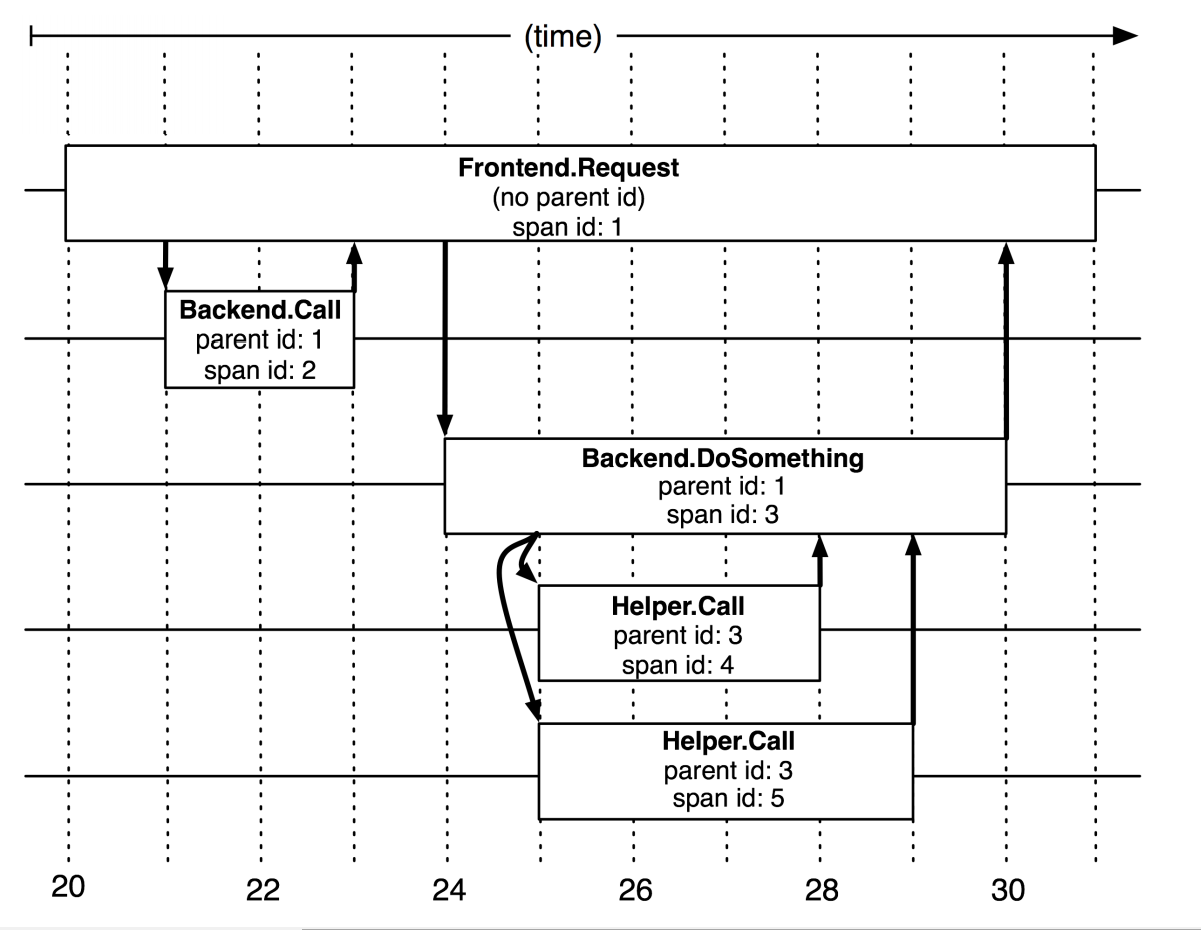
\includegraphics[scale=1]{dappertrace}
            \caption{The relationships between traces in a trace tree}
            \label{fig:dappertrace}
        \end{figure}

        As described thus far, Dapper trace trees allow for a detailed view of the relationships of distributed systems within
        Google. When using this data for debugging or performance analysis, it can often be convenient or even necessary to 
        have additional context surrounding a trace tree or its individual spans. As such, the paper describes a simple API 
        through which application developers can provide a combination of two types of annotations: timestamped textual annotations
        and key-value, allowing for defining arbitrary equivalence classes between traces which can be operated upon in the analysis
        tools.


        \subsection{OpenTracing}

        \newpage


    \section{Main Chapter}

    \subsection{No}

    \section{Conclusion}
    
\end{document}